\mode*
\subsection{Attente et signalement}
\begin{frame}[fragile]{Attente et signalement}
  \begin{tikzpicture}
%    \fill[alertColor!20, rounded corners] (4,6.52) rectangle (6.4,6.82);


    \fill[structure!20, rounded corners] (3.5,3.5) rectangle (8.5,4.15);
    \draw[structure] (11,3.85) node{//$T_{reader}$};

    \draw<2>[alertColor, thick] (3.6,4.03) -- (7.7,4.03);
    \draw<2>[alertColor, thick] (7,4.2) node[above right]{Comment supprimer l'attente active ?};

    \fill[exampleColor!20, rounded corners] (5.1,1.85) rectangle (8.5,2.15);
    \draw[exampleColor] (11,2) node{//$T_{writer}$};
    \draw (5,4.85) node{\begin{minipage}{5cm}\begin{lstlisting}[numbers=none]
class Counter {
  private int value=0;
  public synchronized void increment() {
    ++value;
  }
  public synchronized int get() {
    return value;
  }

  public static void main(String[] args) {
    var counter = new Counter();
    
    new Thread(() -> {
      while(counter.get()==0);
      System.out.println("done");
    }).start();
    
    Thread.sleep(250);
   
    new Thread(counter::increment).start();
  }
}
\end{lstlisting}\end{minipage}};
  \end{tikzpicture}
\end{frame}

\begin{frame}{Sémaphore}
  \begin{center}
    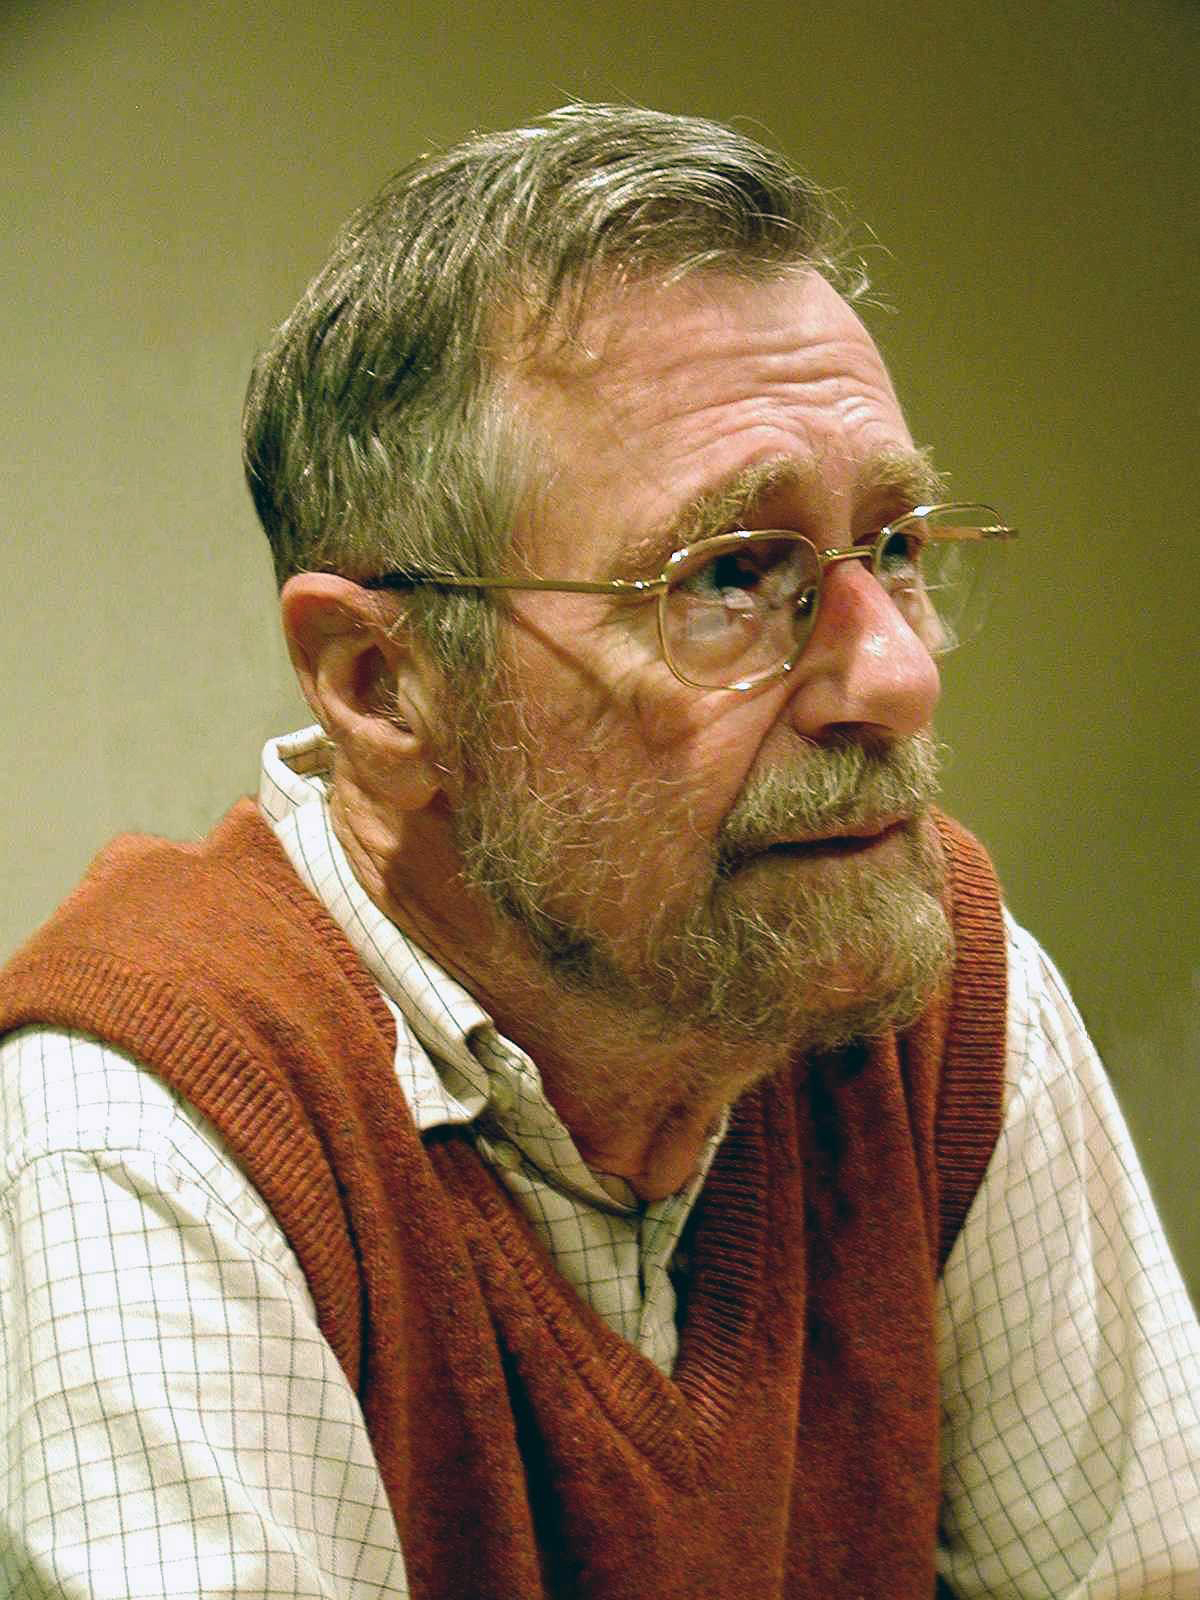
\includegraphics[height=2cm]{Dijkstra}\\
    Edsger W. Dijkstra
  \end{center}
  \vFill
  \begin{block}{Classe \lstinline{java.util.concurrent.Semaphore}}
      \begin{itemize}
      \item \lstinline{new Semaphore(n)}
	\begin{enumerate}
	\item Initialise un sémaphore avec $n$ jetons
	\end{enumerate}
      \item \lstinline{public void acquire() throws InterruptedException}
	\begin{enumerate}
	\item S'il reste un jeton, donner un jeton.
	\item Sinon, attendre qu'un jeton se libère.
	\end{enumerate}
      \item \lstinline{public void release()}
	\begin{enumerate}
	\item Libérer un jeton.
	\end{enumerate}
      \end{itemize}
  \end{block}
  \vFill
  \begin{citing}
  \item[D62] Edsger W. Dijkstra. \textit{Over de sequentialiteit van procesbeschrijvingen (About the sequentiality of process descriptions)} (1962-1963)
  \end{citing}
\end{frame}


\begin{frame}[fragile]{Signalement par sémaphore}
  \begin{tikzpicture}
    \draw (5,4.85) node{\begin{minipage}{5cm}\begin{lstlisting}[numbers=none]
public static void main(String[] args) {
  var semaphore = new Semaphore(0);
  
  new Thread(() -> {
    semaphore.acquire();
    System.out.println("done");
  }).start();
  
  Thread.sleep(250);
 
  new Thread(semaphore::release).start();
}
\end{lstlisting}\end{minipage}};
  \end{tikzpicture}
\end{frame}

\subsection{Notion de moniteur}

\begin{frame}{Moniteur}

  \vFill
  \begin{block}{Construction de synchronisation}
    \begin{itemize}
    \item Un moniteur est un objet encapsulant des données partagées.
    \item Accès aux données partagées en exclusion mutuelle.
    \item Méthodes gardées par des conditions bloquantes (gardes).
    \end{itemize}
  \end{block}

  \vFill
  \hFill
  \begin{minipage}{.4\textwidth}
    \begin{center}
      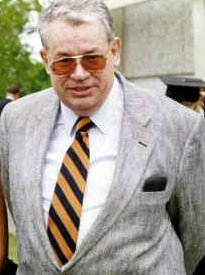
\includegraphics[height=3cm]{hansen}\\
      Per Brinch Hansen
    \end{center}
  \end{minipage}
  \hFill
  \begin{minipage}{.5\textwidth}
    \begin{center}
      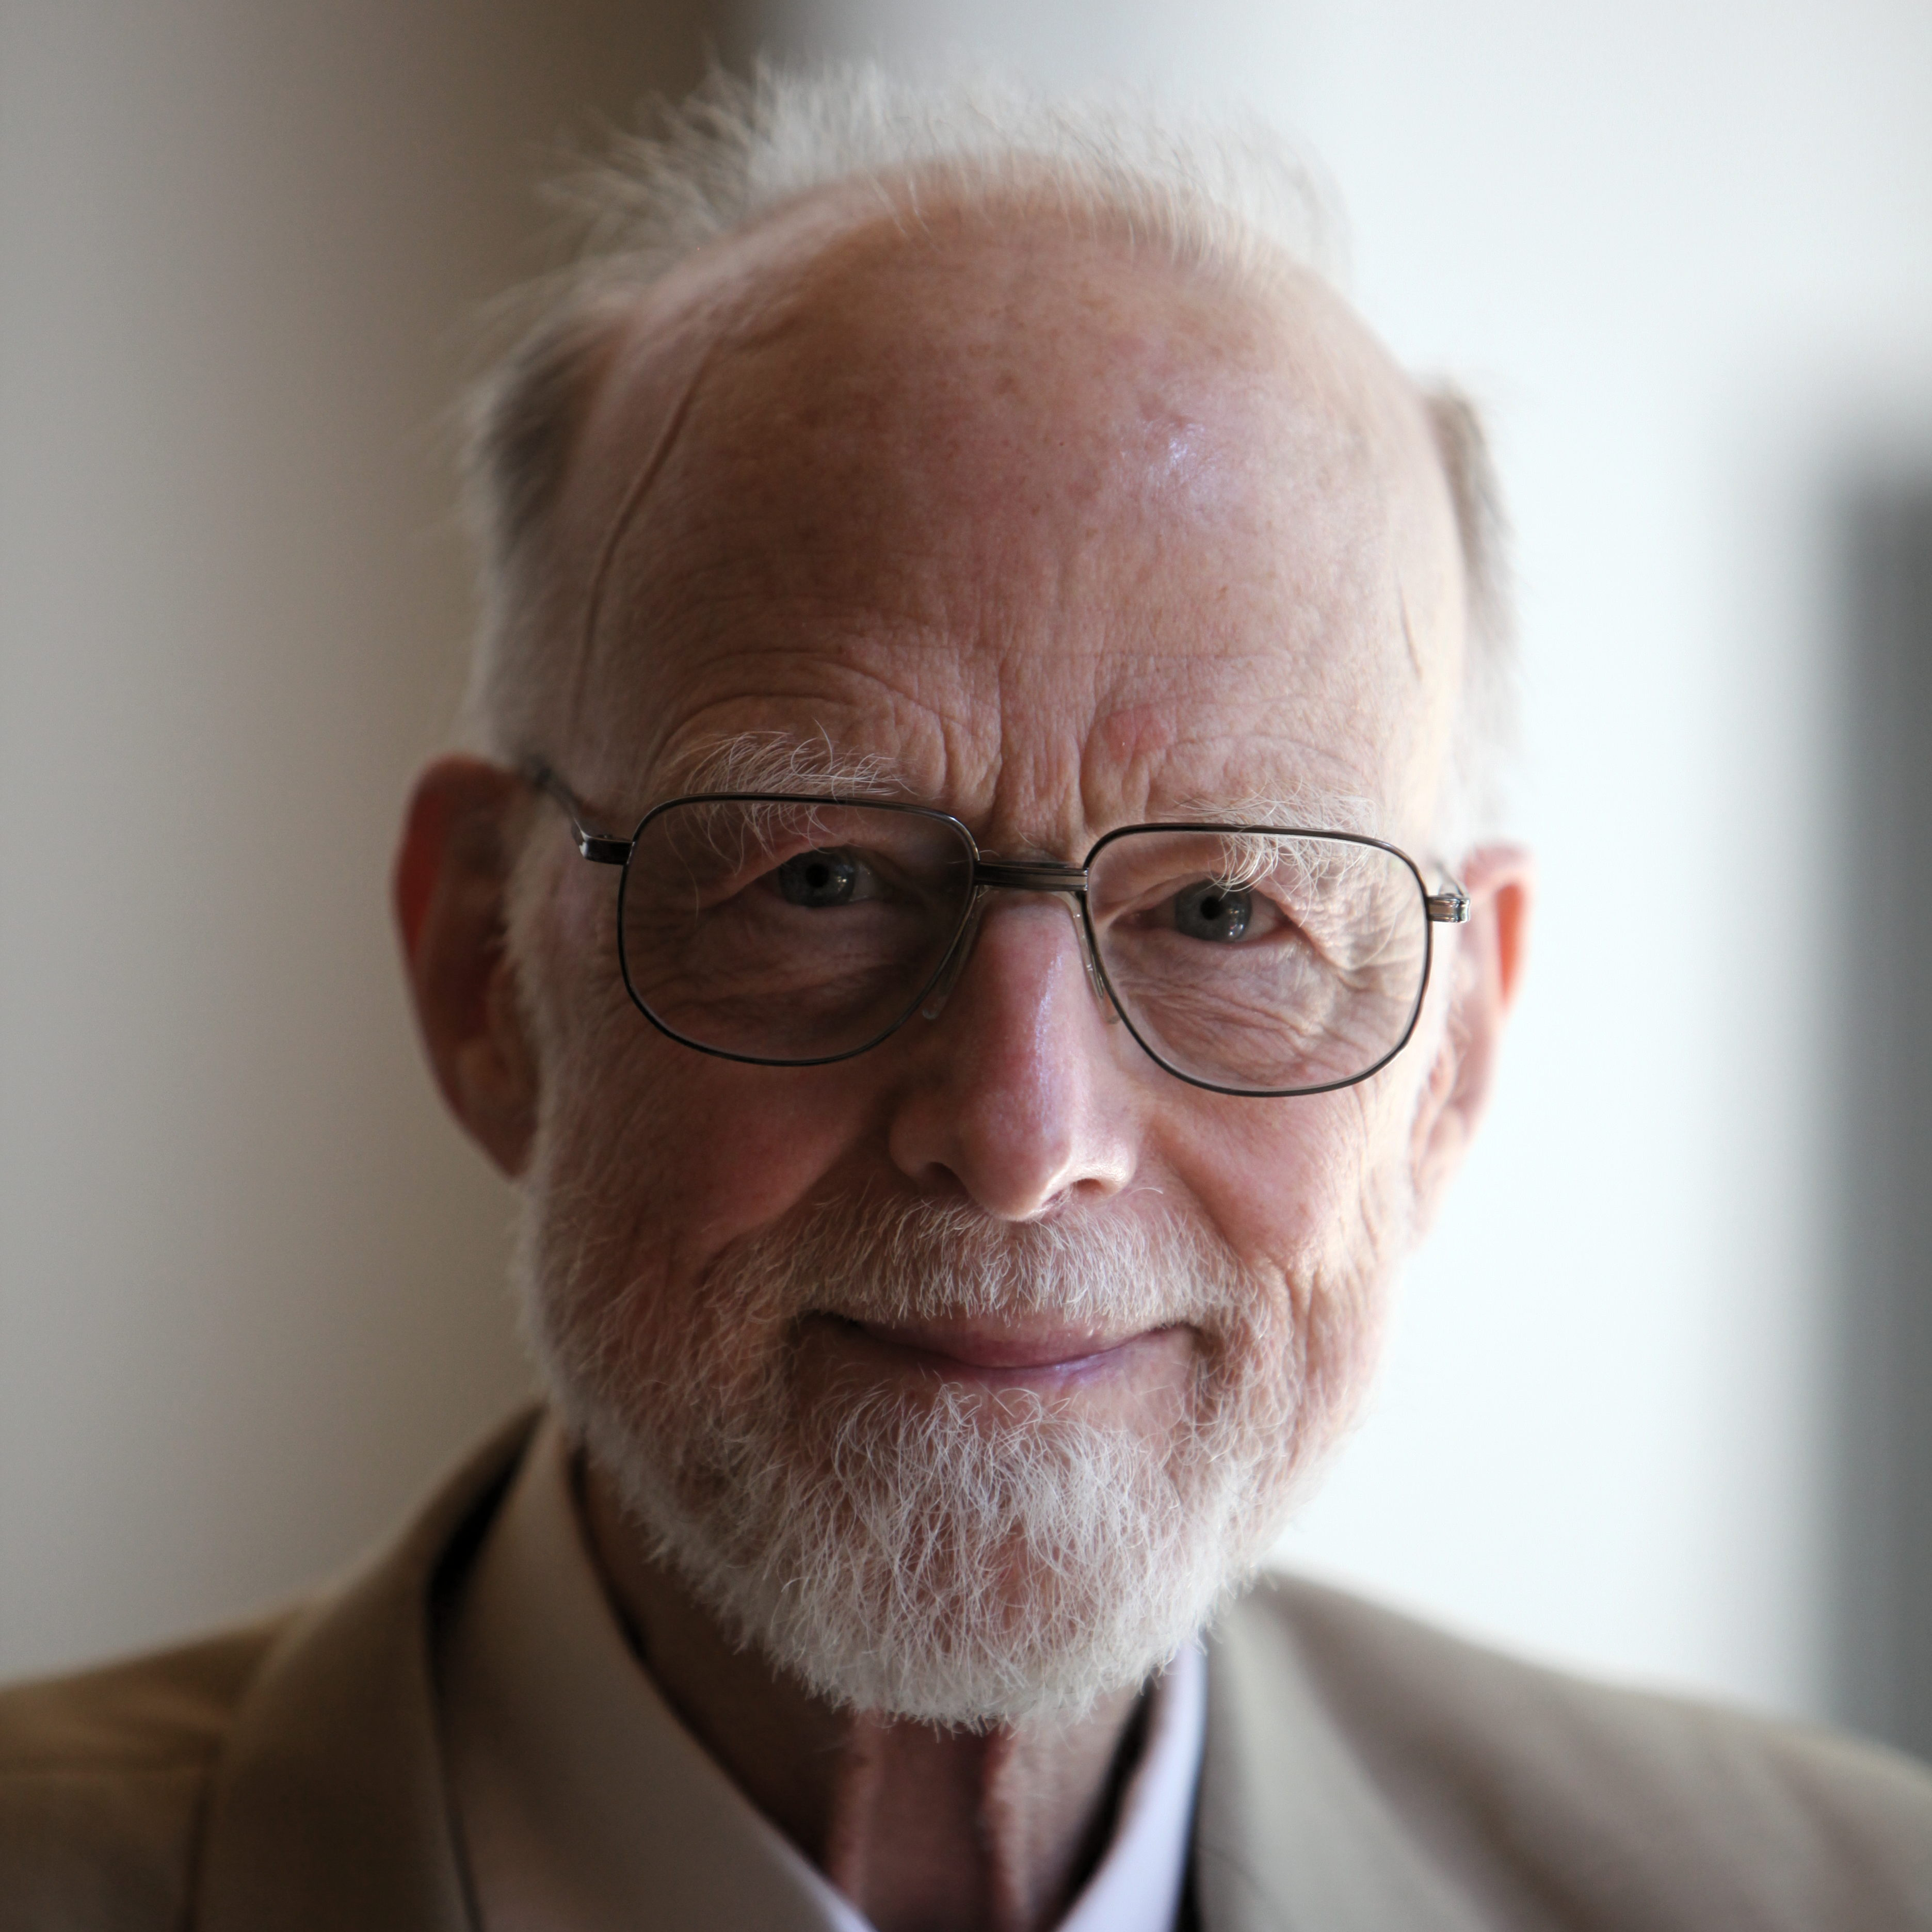
\includegraphics[height=3cm]{hoare}\\
      Tony Hoare
    \end{center}
  \end{minipage}
  \hFill

  \vFill
  \begin{citing}
  \item[] Per Brinch Hansen. \textit{Operating System Principles}. Prentice Hall (1973)
  \item[H74] C. A. R. Hoare. \textit{Monitors: an operating system structuring concept}. CACM (1974)
  \end{citing}
\end{frame}

%%%%%%%%%%%%%%%%%%%%%%%%%%%%%%%%%%%%%%%%%%%%%%%%%%%%%%%%%%%%%%%%%%%%%%%%% 

\begin{frame}{File bloquante}

\vfill
  \begin{exampleblock}{Interface \lstinline{java.util.concurrent.BlockingQueue}}~

\vfill

~\hspace{-5mm}\begin{tabular}{|l|l|l|l|l|}
      \hline
      & Exception & Valeur spéciale & Bloquante & Timeout\\
      \hline
      Insérer & \lstinline+add(e)+ & \lstinline+offer(e)+ & \lstinline+put(e)+ & \lstinline+offer(e, time, unit)+  \\
      \hline
      Supprimer & \lstinline+remove()+ & \lstinline+poll()+ & \lstinline+take()+ & \lstinline+poll(time, unit)+ \\
      \hline
      Regarder & \lstinline+element()+ & \lstinline+peek()+ &  &  \\
      \hline
    \end{tabular}
  \end{exampleblock}

\vfill
\end{frame}

\begin{frame}[fragile]{Le problème des producteurs et des consommateurs}
\vspace{-3mm}
  \begin{tikzpicture}

    \fill[structure!20, rounded corners] (2.8,1.7) rectangle (9.3,4.35);
    \draw[structure] (9.3,3) node[right]{Producteur};
  
    \fill[exampleColor!20, rounded corners] (2.8,5.35) rectangle (9.3,7);
    \draw[exampleColor] (9.3,6.2) node[right]{Consommateur};

    \fill[fill=alertColor!20, rounded corners] (2.8,1.7) rectangle (6,2);
    \fill[fill=alertColor!20, rounded corners] (3.1,3.35) rectangle (6.3,3.65);
    \fill[fill=alertColor!20, rounded corners] (3.1,6.05) rectangle (7,6.35);
    \fill[fill=alertColor!20, rounded corners] (2.4,8.05) rectangle (7.6,8.35);

    \draw (5,4.85) node{\begin{minipage}{5cm}\begin{lstlisting}[numbers=none]
BlockingQueue<Integer> queue
  = new LinkedBlockingQueue<Integer>();

new Thread(() -> {
  int value = 1;
  do {
    value = queue.take();
    System.out.println(value);
  } while(value != 1);
}).start();

new Thread(() -> {
  int value = 17;
  while(value != 1) {
    queue.put(value);
    if(value%2 == 0) value = value/2;
    else value = value*3+1;
    Thread.sleep(500);
  }
  queue.put(value);
}).start();
\end{lstlisting}\end{minipage}};
  \end{tikzpicture}

\vspace{-3mm}
\begin{citing}
\jitem \lstinline{ProducerConsumer.java}
\end{citing}
\end{frame}


%%%%%%%%%%%%%%%%%%%%%%%%%%%%%%%%%%%%%%%%%%%%%%%%%%%%%%%%%%%%%%%%%%%%%%%%% 

\begin{frame} 
  \frametitle{Barrières de synchronisation}

  \begin{exampleblock}{Classe \lstinline+java.util.concurrent.CountDownLatch+}
    \begin{itemize}
    \item \lstinline+public void await() throws InterruptedException+\\
      \begin{itemize}
      \item Se met en attente jusqu'à ce que le compteur atteigne 0
      \end{itemize}
      \medskip
    \item \lstinline+public void countDown()+\\
      \begin{itemize}
      \item Décrémente le compteur
      \end{itemize}
    \end{itemize}
  \end{exampleblock}

  \bigskip
  
  \begin{exampleblock}{Classe \lstinline{java.util.concurrent.CyclicBarrier}}
    \begin{itemize}
    \item\lstinline{public int await() throws InterruptedException, BrokenBarrierExc.}\\
      \begin{itemize}
      \item Se met en attente jusqu'à ce que tous les threads aient rejoint la barrière
      \item Quand tous les threads ont rejoint la barrière, les threads sont réveillés et la barrière est réinitialisée.
      \end{itemize}
      \end{itemize}
  \end{exampleblock}
  
\end{frame}

\subsection{Implémentation}

\begin{frame}[fragile]{Le moniteur universel en Java (\lstinline|java.lang.Object|)}

\vfill    
  \begin{block}{\lstinline|public final void java.lang.Object.wait() throws InterruptedException|}
    \begin{itemize}
    \item Met le thread en attente sur l'objet verrouillé.
    \item Il doit \alert{posséder} le verrou de l'objet sur lequel il se met en attente.
    \item Lorsqu'il entre en attente, il \alert{relâche}  le verrou.
    \end{itemize}
  \end{block}

\vfill    
  \begin{block}{\lstinline|public final void java.lang.Object.notify()|}
    \begin{itemize}
    \item Réveille un des threads en attente sur l'objet verrouillé.
    \item Le thread réveillé doit \alert{acquérir} le verrou.
    \end{itemize}
  \end{block}

\vfill    
  \begin{block}{\lstinline|public final void java.lang.Object.notifyAll()|}
    \begin{itemize}
    \item Pareil mais réveille tous les threads en attente sur l'objet verrouillé.
    \end{itemize}
  \end{block}
\vfill
  \begin{alertblock}{Point vocabulaire}
    \begin{itemize}
    \item Un thread demandant l'accès à un code déjà verrouillé est \alert{bloqué}.
    \item Un  thread qui  est mis  en pause  par l'opération wait est \alert{en attente}.      
    \end{itemize}
  \end{alertblock}
\vfill
\end{frame}


\begin{frame}[fragile]{Implémentation d'un sémaphore}
 
  \begin{lstlisting}
class Semaphore {
  private int counter;
  
  public Semaphore( int counter ) {
    this.counter = counter;
  }
 
  synchronized public void acquire()
  throws InterruptedException {
    while(counter <= 0) wait();
    --counter;
  }
  
  synchronized public void release() {
    ++counter;
    notify();
  }
}
\end{lstlisting}
\end{frame}

\begin{frame}[fragile]{Syntaxes alternatives}
  \begin{block}{En Java : \href{https://docs.oracle.com/javase/7/docs/api/java/util/concurrent/locks/Condition.html}{\lstinline{java.util.concurrent.locks.Condition}}}
\begin{lstlisting}
Lock lock = new ReentrantLock();
Condition condition = lock.newCondition(); 

lock.lock();
condition.signal();
condition.await();
lock.unlock();
\end{lstlisting}
\end{block}
  \begin{block}{En C++ : \href{http://www.cplusplus.com/reference/condition_variable/condition_variable/}{\lstinline{std::condition_variable}}}
\begin{lstlisting}
mutex mtx;
condition_variable condition;

unique_lock<mutex> lock(mtx);
condition.notify_one();
condition.wait(lock);
// unlock on ~unique_lock
\end{lstlisting}
\end{block}
\end{frame}

\mode<all>
